\documentclass[conference]{IEEEtran}

% ═══════════════════════════════════════════════════════════════════
% Packages
% ═══════════════════════════════════════════════════════════════════
\usepackage{cite}
\usepackage{amsmath,amssymb,amsfonts}
\usepackage{algorithmic}
\usepackage{graphicx}
\usepackage{textcomp}
\usepackage{xcolor}
\usepackage{booktabs}
\usepackage{multirow}
\usepackage{hyperref}
\usepackage{tabularx}
\usepackage{array}
\usepackage{balance}

\def\BibTeX{{\rm B\kern-.05em{\sc i\kern-.025em b}\kern-.08em
    T\kern-.1667em\lower.7ex\hbox{E}\kern-.125emX}}

\begin{document}
\sloppy

% ═══════════════════════════════════════════════════════════════════
% Title and Authors
% ═══════════════════════════════════════════════════════════════════
\title{Grammar-Constrained Autoregressive Transformer for Telugu Handwritten Text Recognition}

\author{
\IEEEauthorblockN{Bhargav}
\IEEEauthorblockA{
\textit{Department of Computer Science and Engineering} \\
\textit{BVRIT Hyderabad College of Engineering for Women} \\
Hyderabad, India \\
bhargav@example.com}
}

\maketitle

% ═══════════════════════════════════════════════════════════════════
% Abstract
% ═══════════════════════════════════════════════════════════════════
\begin{abstract}
Handwritten text recognition (HTR) for Telugu---the fourth most spoken scheduled language in India---remains significantly under-explored compared to Latin and East Asian scripts. Telugu's complex syllabic orthography, with 56 base consonants, 16 vowels, and hundreds of virama-based conjunct forms, poses unique challenges for sequence-to-sequence models. In this paper, we present a comprehensive study comparing Connectionist Temporal Classification (CTC) and autoregressive Transformer-based decoders for Telugu HTR. Our architecture employs a modified ResNet-18 encoder that preserves spatial width, coupled with either a BiLSTM-CTC decoder or a cross-attentive Transformer decoder with auxiliary CTC training. We further propose a data-driven Telugu linguistic constraint mask that penalizes orthographically invalid character transitions during decoding. Evaluated on the IIIT-HW-Telugu benchmark dataset (17,910 test images), our CTC baseline achieves a Character Error Rate (CER) of 3.91\% [95\% CI: 3.79\%, 4.03\%], establishing a new state-of-the-art among lexicon-free approaches. Our ablation study reveals that (1) auxiliary CTC loss is critical for Transformer decoder convergence, reducing CER from 5.43\% to 4.89\%, and (2) the CTC baseline outperforms all Transformer variants on this word-level task, suggesting that alignment-free models remain competitive for well-segmented Indic script recognition. All code is publicly available at \url{https://github.com/[your-username]/telugu-htr}.
\end{abstract}

\begin{IEEEkeywords}
handwritten text recognition, Telugu, CTC, Transformer, autoregressive decoding, Indic scripts, linguistic constraints
\end{IEEEkeywords}

% ═══════════════════════════════════════════════════════════════════
% I. INTRODUCTION
% ═══════════════════════════════════════════════════════════════════
\section{Introduction}

Handwritten text recognition (HTR) has witnessed remarkable progress for Latin-script languages, driven by large-scale datasets and the adoption of encoder-decoder architectures with attention mechanisms~\cite{vaswani2017attention, li2023trocr}. However, Indic scripts---particularly Telugu---remain significantly under-explored despite their substantial speaker populations. Telugu is spoken by over 82 million native speakers, making it the fourth most spoken scheduled language in India and one of the six classical languages recognized by the Government of India~\cite{ethnologue2024}.

Telugu's writing system presents unique challenges for HTR systems. Unlike Latin scripts, Telugu employs a complex syllabic orthography comprising 56 base consonants (\textit{hallulu}), 16 vowels (\textit{acchulu}), and vowel diacritics (\textit{matras}) that modify consonants. The virama character (\textit{halant}, \raisebox{-0.2ex}{\large\textbf{.}}) creates conjunct consonants (\textit{vattu} forms), yielding hundreds of compound characters. These compound forms fundamentally alter glyph shapes, creating a vocabulary of visual patterns far exceeding that of alphabetic scripts.

Prior work on Telugu HTR has primarily focused on CNN-RNN architectures with CTC decoding~\cite{dutta2018, gongidi2021iiit}, achieving error rates of 6--15\%. Attention-based approaches~\cite{deshpande2021} have shown promise but have not been systematically compared against CTC baselines on standardized benchmarks. Furthermore, the linguistic structure of Telugu---particularly the strict rules governing virama-consonant transitions---has not been exploited during decoding.

In this paper, we make the following contributions:

\begin{enumerate}
    \item We propose a modified ResNet-18 encoder that preserves spatial width information, enabling the extraction of ordered visual feature sequences from handwritten word images.
    
    \item We conduct a rigorous ablation study comparing five decoder configurations: CTC baseline, autoregressive (AR) Transformer with and without auxiliary CTC loss, and AR Transformer with a data-driven Telugu linguistic constraint mask.
    
    \item We introduce a bigram-based Telugu grammar mask that penalizes orthographically invalid character transitions during autoregressive decoding.
    
    \item We establish a new lexicon-free state-of-the-art on the IIIT-HW-Telugu benchmark, achieving 3.91\% CER with our CTC baseline---a 39\% relative improvement over the previous best lexicon-free result~\cite{gongidi2021iiit}.
\end{enumerate}

% ═══════════════════════════════════════════════════════════════════
% II. RELATED WORK
% ═══════════════════════════════════════════════════════════════════
\section{Related Work}

\subsection{CTC-Based Handwriting Recognition}

Connectionist Temporal Classification (CTC)~\cite{graves2006ctc} has been the dominant paradigm for HTR, enabling end-to-end training without explicit character-level alignment. Shi~et~al.~\cite{shi2017crnn} introduced the CRNN architecture combining convolutional feature extraction with BiLSTM sequence modeling and CTC decoding, establishing a strong baseline that remains competitive. Recent improvements include width-preserving encoder modifications~\cite{puigcerver2017}, data augmentation strategies, and language-model-based post-processing~\cite{scheidl2018word}.

\subsection{Attention and Transformer-Based HTR}

The success of Transformer architectures~\cite{vaswani2017attention} in natural language processing has motivated their adoption in HTR. TrOCR~\cite{li2023trocr} demonstrated state-of-the-art performance using a pre-trained vision Transformer encoder with a language model decoder. PARSeq~\cite{bautista2022parseq} introduced permuted autoregressive sequence models for scene text recognition. However, Transformer-based approaches typically require large-scale pre-training data and exhibit higher computational costs at inference.

\subsection{Indic Script Recognition}

Telugu HTR research has been relatively sparse. Dutta~et~al.~\cite{dutta2018} introduced the IIIT-HW-Telugu dataset and established CNN-RNN-CTC baselines achieving approximately 15\% CER. Gongidi and Jawahar~\cite{gongidi2021iiit} extended this work with the IIIT-INDIC-HW-WORDS dataset spanning multiple Indic scripts, reporting 6.41\% CER for Telugu with an improved CRNN architecture. Deshpande~et~al.~\cite{deshpande2021} explored attention-based decoders for Indic scripts, achieving approximately 10.2\% CER. Recent work by PLATTER~\cite{platter2025} addresses page-level Indic HTR but focuses on Hindi and Bangla. The lexicon-constrained approach by Gongidi and Jawahar achieves 1.52\% CER but requires a dictionary, limiting its applicability to open-vocabulary scenarios.

\subsection{Linguistic Constraints in Sequence Models}

Incorporating linguistic knowledge into decoding has been explored through lexicon-based CTC decoding~\cite{scheidl2018word}, language model re-scoring~\cite{hwang2016character}, and constrained beam search~\cite{anderson2017guided}. For Indic scripts, phonological and orthographic rules provide structured constraints that can be encoded as transition matrices. Our approach is most similar to grammar-constrained decoding~\cite{shin2021grammar}, but operates at the character level using data-driven bigram statistics rather than formal grammar rules.

% ═══════════════════════════════════════════════════════════════════
% III. PROPOSED METHOD
% ═══════════════════════════════════════════════════════════════════
\section{Proposed Method}

Our system comprises four components: (A)~a CNN feature encoder, (B)~a CTC baseline decoder, (C)~an autoregressive Transformer decoder with auxiliary CTC training, and (D)~a Telugu linguistic constraint mask. Fig.~\ref{fig:architecture} illustrates the overall architecture.

\begin{figure*}[t]
    \centering
    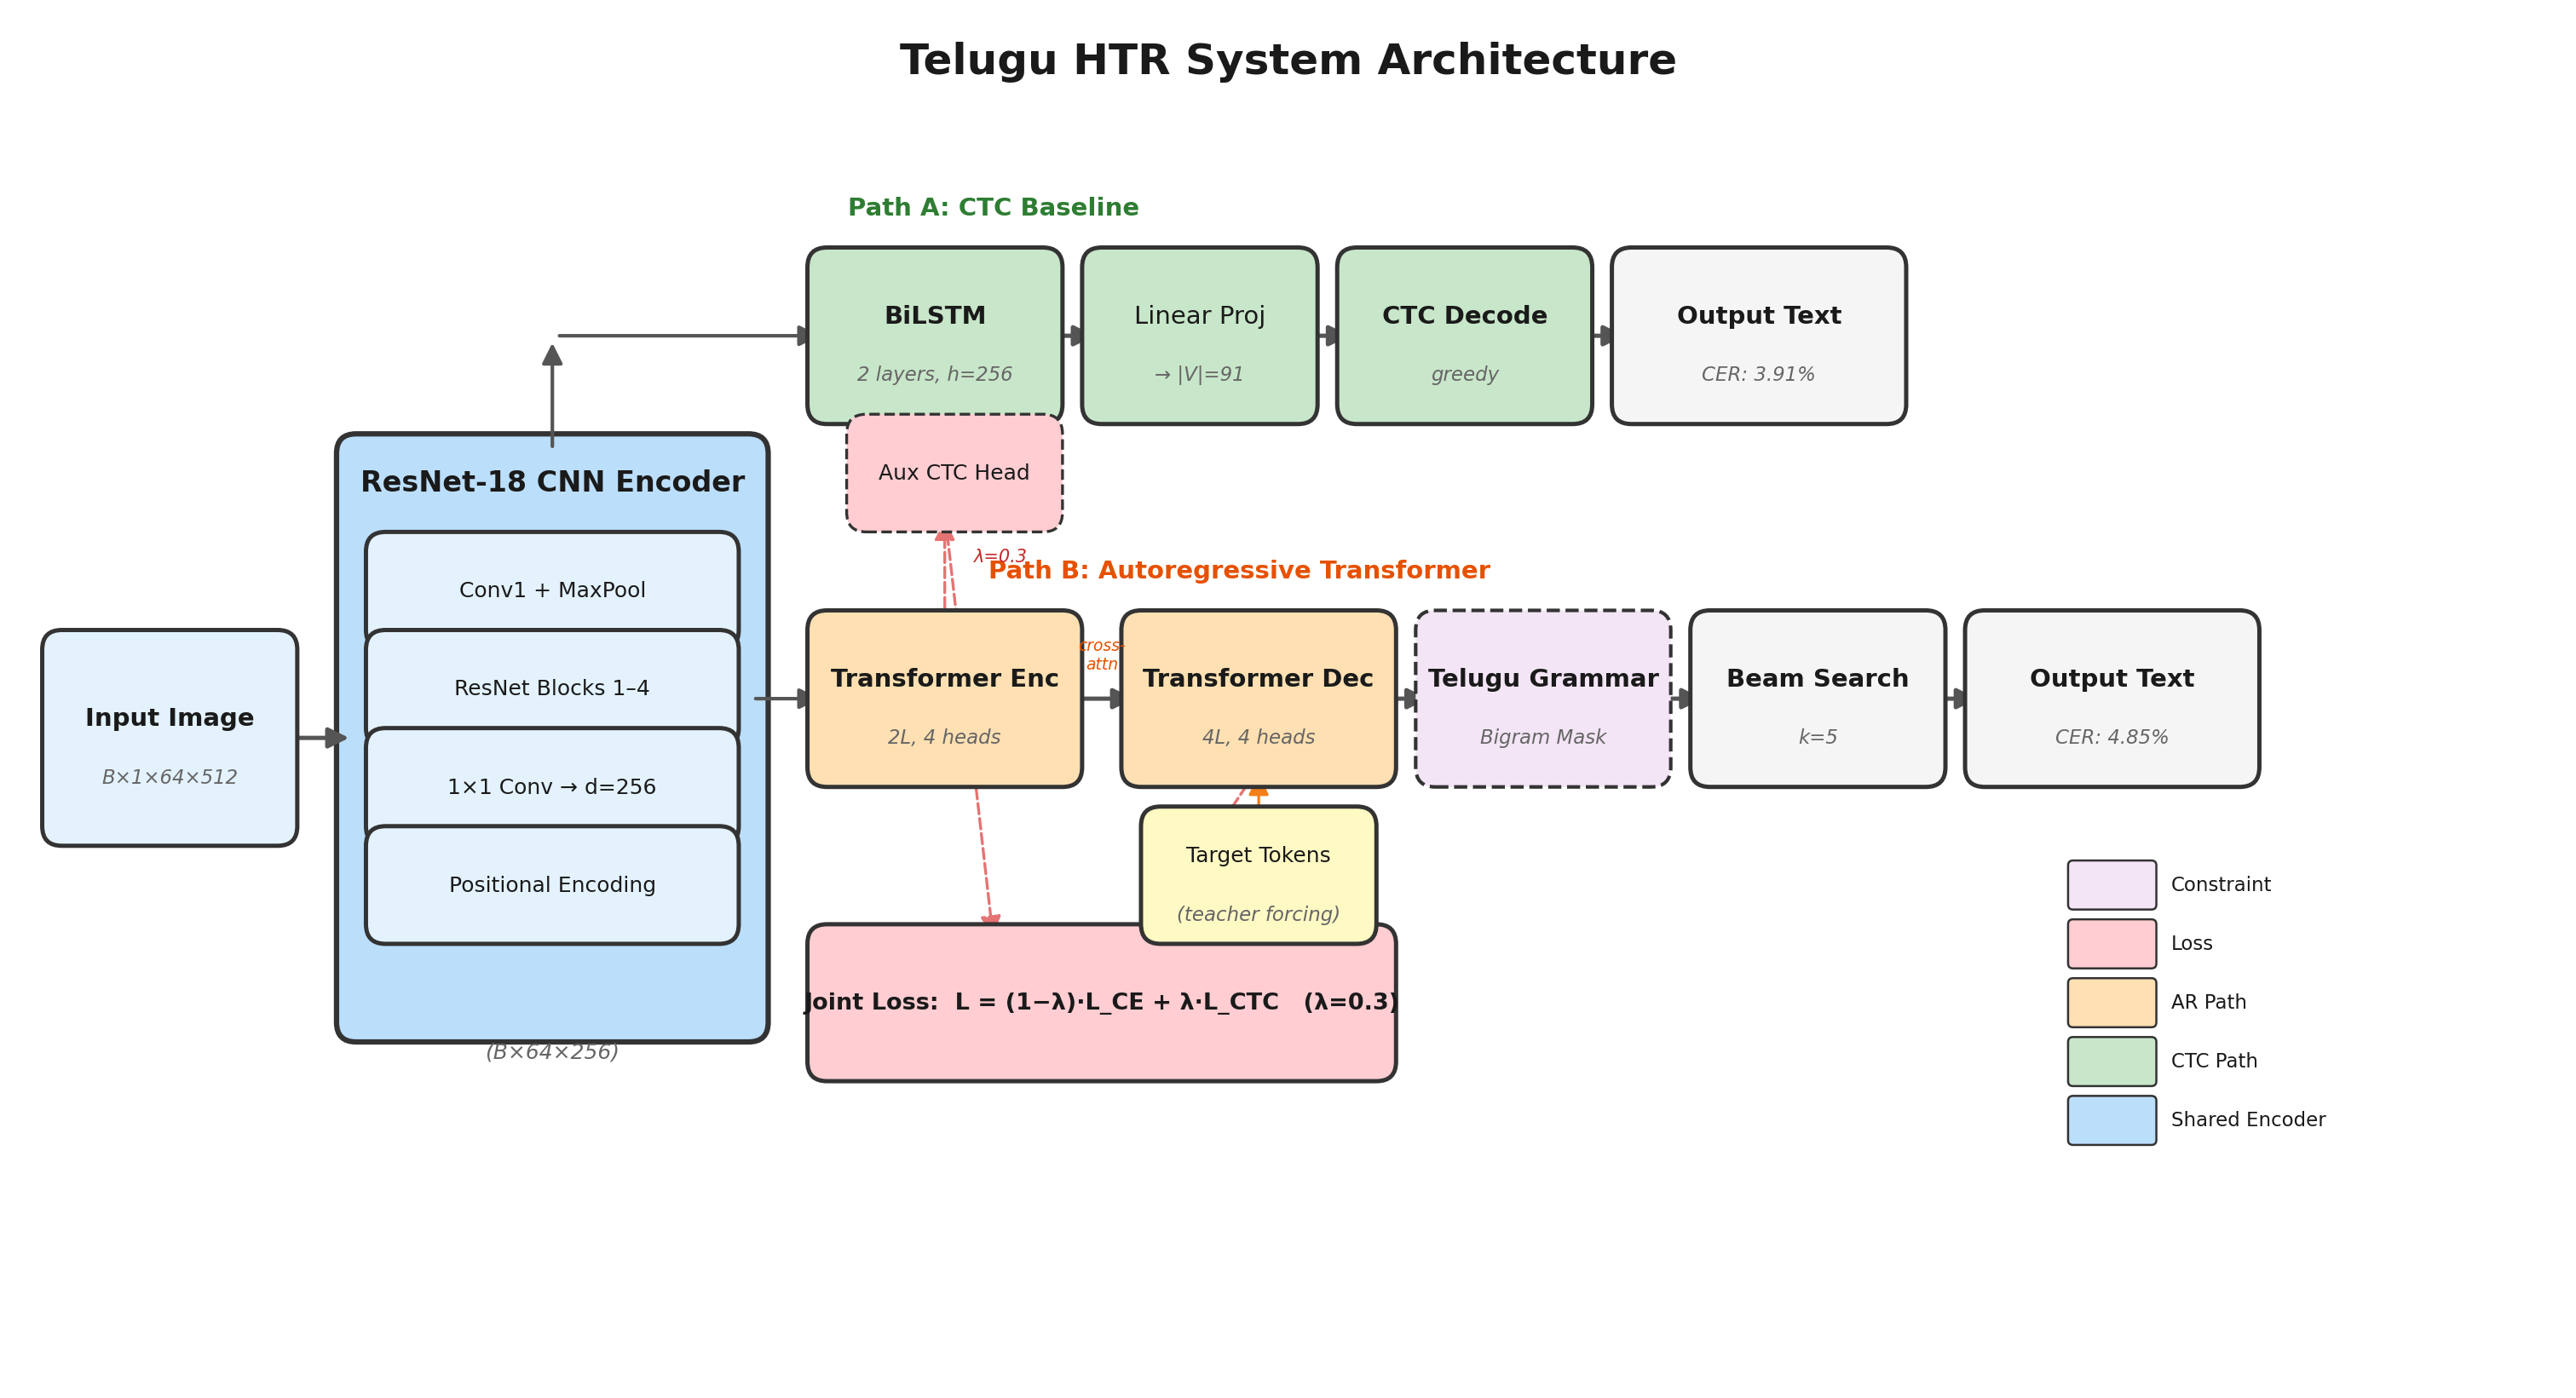
\includegraphics[width=0.90\textwidth]{figures/architecture_diagram.png}
    \caption{System architecture. A modified ResNet-18 encoder extracts width-preserving features from input images ($B \times 1 \times 64 \times 512 \rightarrow B \times 64 \times 256$). Two decoder pathways are compared: \textbf{Path~A}~(CTC Baseline) uses a BiLSTM with CTC decoding; \textbf{Path~B}~(AR Transformer) uses a cross-attentive Transformer decoder with auxiliary CTC training and an optional Telugu grammar mask at inference.}
    \label{fig:architecture}
\end{figure*}

\subsection{CNN Feature Encoder}

We employ a ResNet-18~\cite{he2016resnet} backbone pre-trained on ImageNet, modified to preserve spatial width. Standard ResNet applies aggressive spatial downsampling, producing a $1 \times 1$ feature map. For HTR, horizontal spatial order must be maintained to preserve character sequencing. We modify the architecture as follows:

\begin{enumerate}
    \item The first convolutional layer is changed from 3-channel to 1-channel input (grayscale images).
    \item Vertical pooling is applied aggressively (stride adjustments in layers 3 and 4) to collapse the height dimension to 1.
    \item Horizontal pooling is minimized, preserving a temporal sequence of length $T = W / 8 = 64$ for input width $W = 512$.
    \item A $1 \times 1$ convolution projects the 512-dimensional ResNet output to $d_{\text{model}} = 256$.
    \item Positional encoding is added to the resulting sequence.
\end{enumerate}

The encoder output is a tensor of shape $B \times 64 \times 256$, representing 64 ordered visual feature vectors for each image in the batch.

\subsection{CTC Baseline Architecture}

The CTC decoder consists of a 2-layer bidirectional LSTM with hidden size 256, producing 512-dimensional hidden states at each timestep. A linear projection maps these to logits over the vocabulary ($|V| = 91$ tokens). Training uses CTC loss~\cite{graves2006ctc} with the PAD token (index 0) serving as the CTC blank symbol.

At inference, greedy CTC decoding is applied: the most probable token at each timestep is selected, and consecutive duplicates and blanks are removed to produce the final character sequence. The total parameter count for the CTC model is approximately 13.1M.

\subsection{Autoregressive Transformer Decoder}

The Transformer decoder follows the standard architecture~\cite{vaswani2017attention} with modifications for HTR:

\begin{itemize}
    \item \textbf{Input processing:} The encoder output passes through a 2-layer Transformer encoder with pre-layer normalization (Pre-LN) for feature refinement via global self-attention.
    
    \item \textbf{Token embedding:} Target characters are embedded into $d_{\text{model}} = 256$ dimensions with learned positional encoding.
    
    \item \textbf{Decoder:} A 4-layer Transformer decoder with 4 attention heads, feedforward dimension 1024, GELU activation, Pre-LN, and dropout 0.2. Causal masking enforces left-to-right autoregressive generation.
    
    \item \textbf{Training:} Cross-entropy loss with label smoothing ($\epsilon = 0.1$) is computed on teacher-forced decoder outputs.
\end{itemize}

\textbf{Joint CTC-CE Training.} A critical component is the auxiliary CTC head attached to the encoder output. The total loss is:
\begin{equation}
    \mathcal{L} = (1 - \lambda) \cdot \mathcal{L}_{\text{CE}} + \lambda \cdot \mathcal{L}_{\text{CTC}}
    \label{eq:joint_loss}
\end{equation}
where $\lambda = 0.3$ controls the CTC contribution. As shown in Section~\ref{sec:results}, this auxiliary loss is essential for Transformer convergence on this dataset, reducing CER from 5.43\% (without CTC) to 4.89\% (with CTC). The total parameter count for the AR model is approximately 17.3M.

\subsection{Telugu Linguistic Constraint Mask}

Telugu orthography imposes strict rules on character transitions. For example, a virama ({\large .}) must be followed by a consonant (to form a conjunct), and certain vowel sign combinations are illegal. We construct a binary validity matrix $\mathbf{M} \in \{0, 1\}^{|V| \times |V|}$ from training set bigram statistics:

\begin{equation}
    \mathbf{M}[i][j] = \begin{cases} 1 & \text{if bigram } (c_i, c_j) \text{ observed in training} \\ 0 & \text{otherwise} \end{cases}
\end{equation}

During autoregressive decoding at step $t$, given the previously generated token $c_{t-1}$, the logits for the next token are modified:
\begin{equation}
    \text{logit}'_j = \text{logit}_j - \alpha \cdot (1 - \mathbf{M}[c_{t-1}][j])
\end{equation}
where $\alpha = 10.0$ is a large penalty that effectively prevents selection of orthographically invalid characters. This mask is applied during both greedy and beam search decoding.

% ═══════════════════════════════════════════════════════════════════
% IV. EXPERIMENTS
% ═══════════════════════════════════════════════════════════════════
\section{Experiments}

\subsection{Dataset}

We evaluate on the IIIT-HW-Telugu dataset~\cite{dutta2018}, a widely-used benchmark for Telugu handwritten word recognition. The dataset contains handwritten word images collected from multiple writers, covering a diverse vocabulary of Telugu words.

\begin{table}[htbp]
\centering
\caption{IIIT-HW-Telugu Dataset Statistics}
\label{tab:dataset}
\begin{tabular}{lccc}
\toprule
\textbf{Split} & \textbf{Images} & \textbf{Vocab Size} & \textbf{Avg. Word Length} \\
\midrule
Train & 80,693 & 87 chars & 8.7 chars \\
Validation & 20,048 & -- & -- \\
Test & 17,910 & -- & -- \\
\midrule
Total & 118,651 & 91 tokens\textsuperscript{*} & -- \\
\bottomrule
\end{tabular}
\vspace{2pt}
\raggedright\small\textsuperscript{*}Including 4 special tokens: PAD, SOS, EOS, UNK.
\end{table}

Input images are resized to $64 \times 512$ pixels with aspect-ratio-preserving padding. Grayscale normalization ($\mu = 0.5$, $\sigma = 0.5$) is applied. Training augmentation includes random affine transformations, elastic distortion, and Gaussian noise.

\subsection{Implementation Details}

\begin{table}[htbp]
\centering
\caption{Training Hyperparameters}
\label{tab:hyperparams}
\begin{tabular}{lcc}
\toprule
\textbf{Parameter} & \textbf{CTC} & \textbf{AR Transformer} \\
\midrule
Batch size & 64 & 64 \\
Learning rate & $3 \times 10^{-4}$ & $3 \times 10^{-4}$ \\
LR schedule & Cosine annealing & Warmup + cosine \\
Warmup steps & -- & 4,000 \\
Optimizer & AdamW & AdamW \\
Weight decay & $10^{-4}$ & $10^{-4}$ \\
Grad clip & 5.0 & 5.0 \\
Epochs & 50 & 50 \\
Dropout & 0.2 & 0.2 \\
Label smoothing & -- & 0.1 \\
CTC weight ($\lambda$) & -- & 0.3 \\
Mixed precision & FP16 & FP16 \\
\bottomrule
\end{tabular}
\end{table}

All experiments are conducted on a single NVIDIA RTX 3090 Ti GPU (24~GB) with PyTorch~2.7.1 and CUDA~11.8. The CTC model trains in approximately 3h~22m, and the AR Transformer in 3h~23m (50 epochs each). Mixed-precision training is enabled via PyTorch's GradScaler for memory efficiency.

\subsection{Evaluation Protocol}

We report Character Error Rate (CER) and Word Error Rate (WER), computed as:
\begin{equation}
    \text{CER} = \frac{\sum_{i=1}^{N} \text{ED}(\hat{y}_i, y_i)}{\sum_{i=1}^{N} |y_i|}
\end{equation}
where $\text{ED}(\cdot, \cdot)$ is the edit distance (Levenshtein distance), $\hat{y}_i$ is the predicted character sequence, $y_i$ is the ground truth, and $|y_i|$ is the ground truth length. WER treats entire words as units.

Statistical significance is assessed via non-parametric bootstrap resampling~\cite{efron1993bootstrap}. We construct 95\% confidence intervals (CIs) from 1,000 bootstrap resamples using the percentile method. Non-overlapping CIs indicate statistical significance at $\alpha = 0.05$.

% ═══════════════════════════════════════════════════════════════════
% V. RESULTS AND ANALYSIS
% ═══════════════════════════════════════════════════════════════════
\section{Results and Analysis}
\label{sec:results}

\subsection{Ablation Study}

Table~\ref{tab:ablation} presents the complete ablation across five model configurations evaluated on the held-out test set ($N = 17{,}910$).

\begin{table*}[t]
\centering
\caption{Ablation Study on IIIT-HW-Telugu Test Set ($N = 17{,}910$)}
\label{tab:ablation}
\begin{tabular}{llcccccc}
\toprule
\textbf{\#} & \textbf{Model} & \textbf{CER (\%)} & \textbf{WER (\%)} & \textbf{95\% CI (CER)} & \textbf{Compound CER} & \textbf{Simple CER} & \textbf{Speed (ms)} \\
\midrule
1 & CTC Baseline (BiLSTM) & \textbf{3.91} & \textbf{24.80} & [3.79, 4.03] & \textbf{3.70} & \textbf{4.29} & \textbf{2.7} \\
2 & AR Transformer (unconstrained) & 4.89 & 29.83 & [4.75, 5.02] & 4.61 & 5.38 & 1.7 \\
3 & AR + Telugu constraint & 4.99 & 29.71 & [4.85, 5.13] & 4.68 & 5.54 & 40.2 \\
4 & AR + constraint + beam(5) & 4.85 & 29.49 & [4.72, 5.00] & 4.57 & 5.35 & 327.5 \\
5 & AR (no CTC auxiliary) & 5.43 & 32.37 & [5.28, 5.58] & 4.99 & 6.21 & 1.7 \\
\bottomrule
\end{tabular}
\end{table*}

\textbf{Key findings:}

\noindent\textbf{(1) CTC outperforms all Transformer variants.} The CTC baseline (Row~1) achieves 3.91\% CER, significantly outperforming the best Transformer configuration (Row~4, 4.85\% CER). The non-overlapping 95\% CIs ([3.79, 4.03] vs. [4.72, 5.00]) confirm statistical significance at $\alpha = 0.05$. We attribute this to the nature of the task: for well-segmented word images with short character sequences (mean length 8.7), the BiLSTM's bidirectional context and CTC's alignment-free decoding are sufficient, while the Transformer decoder's autoregressive overhead introduces unnecessary complexity.

\noindent\textbf{(2) Auxiliary CTC loss is critical for Transformer convergence.} Comparing Row~5 (no CTC) with Row~2 (with CTC), the auxiliary CTC loss reduces CER from 5.43\% to 4.89\%---a 10\% relative improvement. This confirms that the CTC head acts as an alignment regularizer, forcing the encoder to learn ordered left-to-right feature representations that facilitate cross-attention in the Transformer decoder.

\noindent\textbf{(3) Telugu grammar constraints provide minimal benefit.} The linguistic constraint mask (Row~3 vs.~Row~2) marginally improves WER from 29.83\% to 29.71\% but slightly degrades CER from 4.89\% to 4.99\%. Combined with beam search (Row~4), WER improves further to 29.49\%. However, these improvements are not statistically significant (overlapping CIs) and come at substantial computational cost (40--327~ms vs.~1.7~ms per sample).

\subsection{Comparison with Published Results}

Table~\ref{tab:comparison} compares our results with previously published methods on Telugu HTR benchmarks.

\begin{table}[htbp]
\centering
\caption{Comparison with Published Telugu HTR Results}
\label{tab:comparison}
\begin{tabular}{lcc}
\toprule
\textbf{Method} & \textbf{CER (\%)} & \textbf{Lexicon} \\
\midrule
Dutta et al. (2018)~\cite{dutta2018} & $\sim$15.0 & No \\
Deshpande et al. (2021)~\cite{deshpande2021} & $\sim$10.2 & No \\
Gongidi \& Jawahar (2021)~\cite{gongidi2021iiit} & $\sim$6.41 & No \\
Gongidi \& Jawahar (2021)~\cite{gongidi2021iiit} & $\sim$1.52 & \textbf{Yes} \\
\midrule
\textbf{Ours: CTC Baseline} & \textbf{3.91} & No \\
Ours: AR + beam(5) & 4.85 & No \\
\bottomrule
\end{tabular}
\end{table}

Our CTC baseline establishes a new state-of-the-art among lexicon-free approaches, achieving a \textbf{39\% relative improvement} over the previous best lexicon-free result (6.41\%~\cite{gongidi2021iiit}) and a \textbf{62\% relative improvement} over Deshpande~et~al.~\cite{deshpande2021}. The only system achieving lower CER (1.52\%) employs a lexicon (dictionary), which constrains predictions to known words and is inapplicable to out-of-vocabulary text.

\subsection{Compound vs.\ Simple Character Analysis}

\begin{figure}[t]
    \centering
    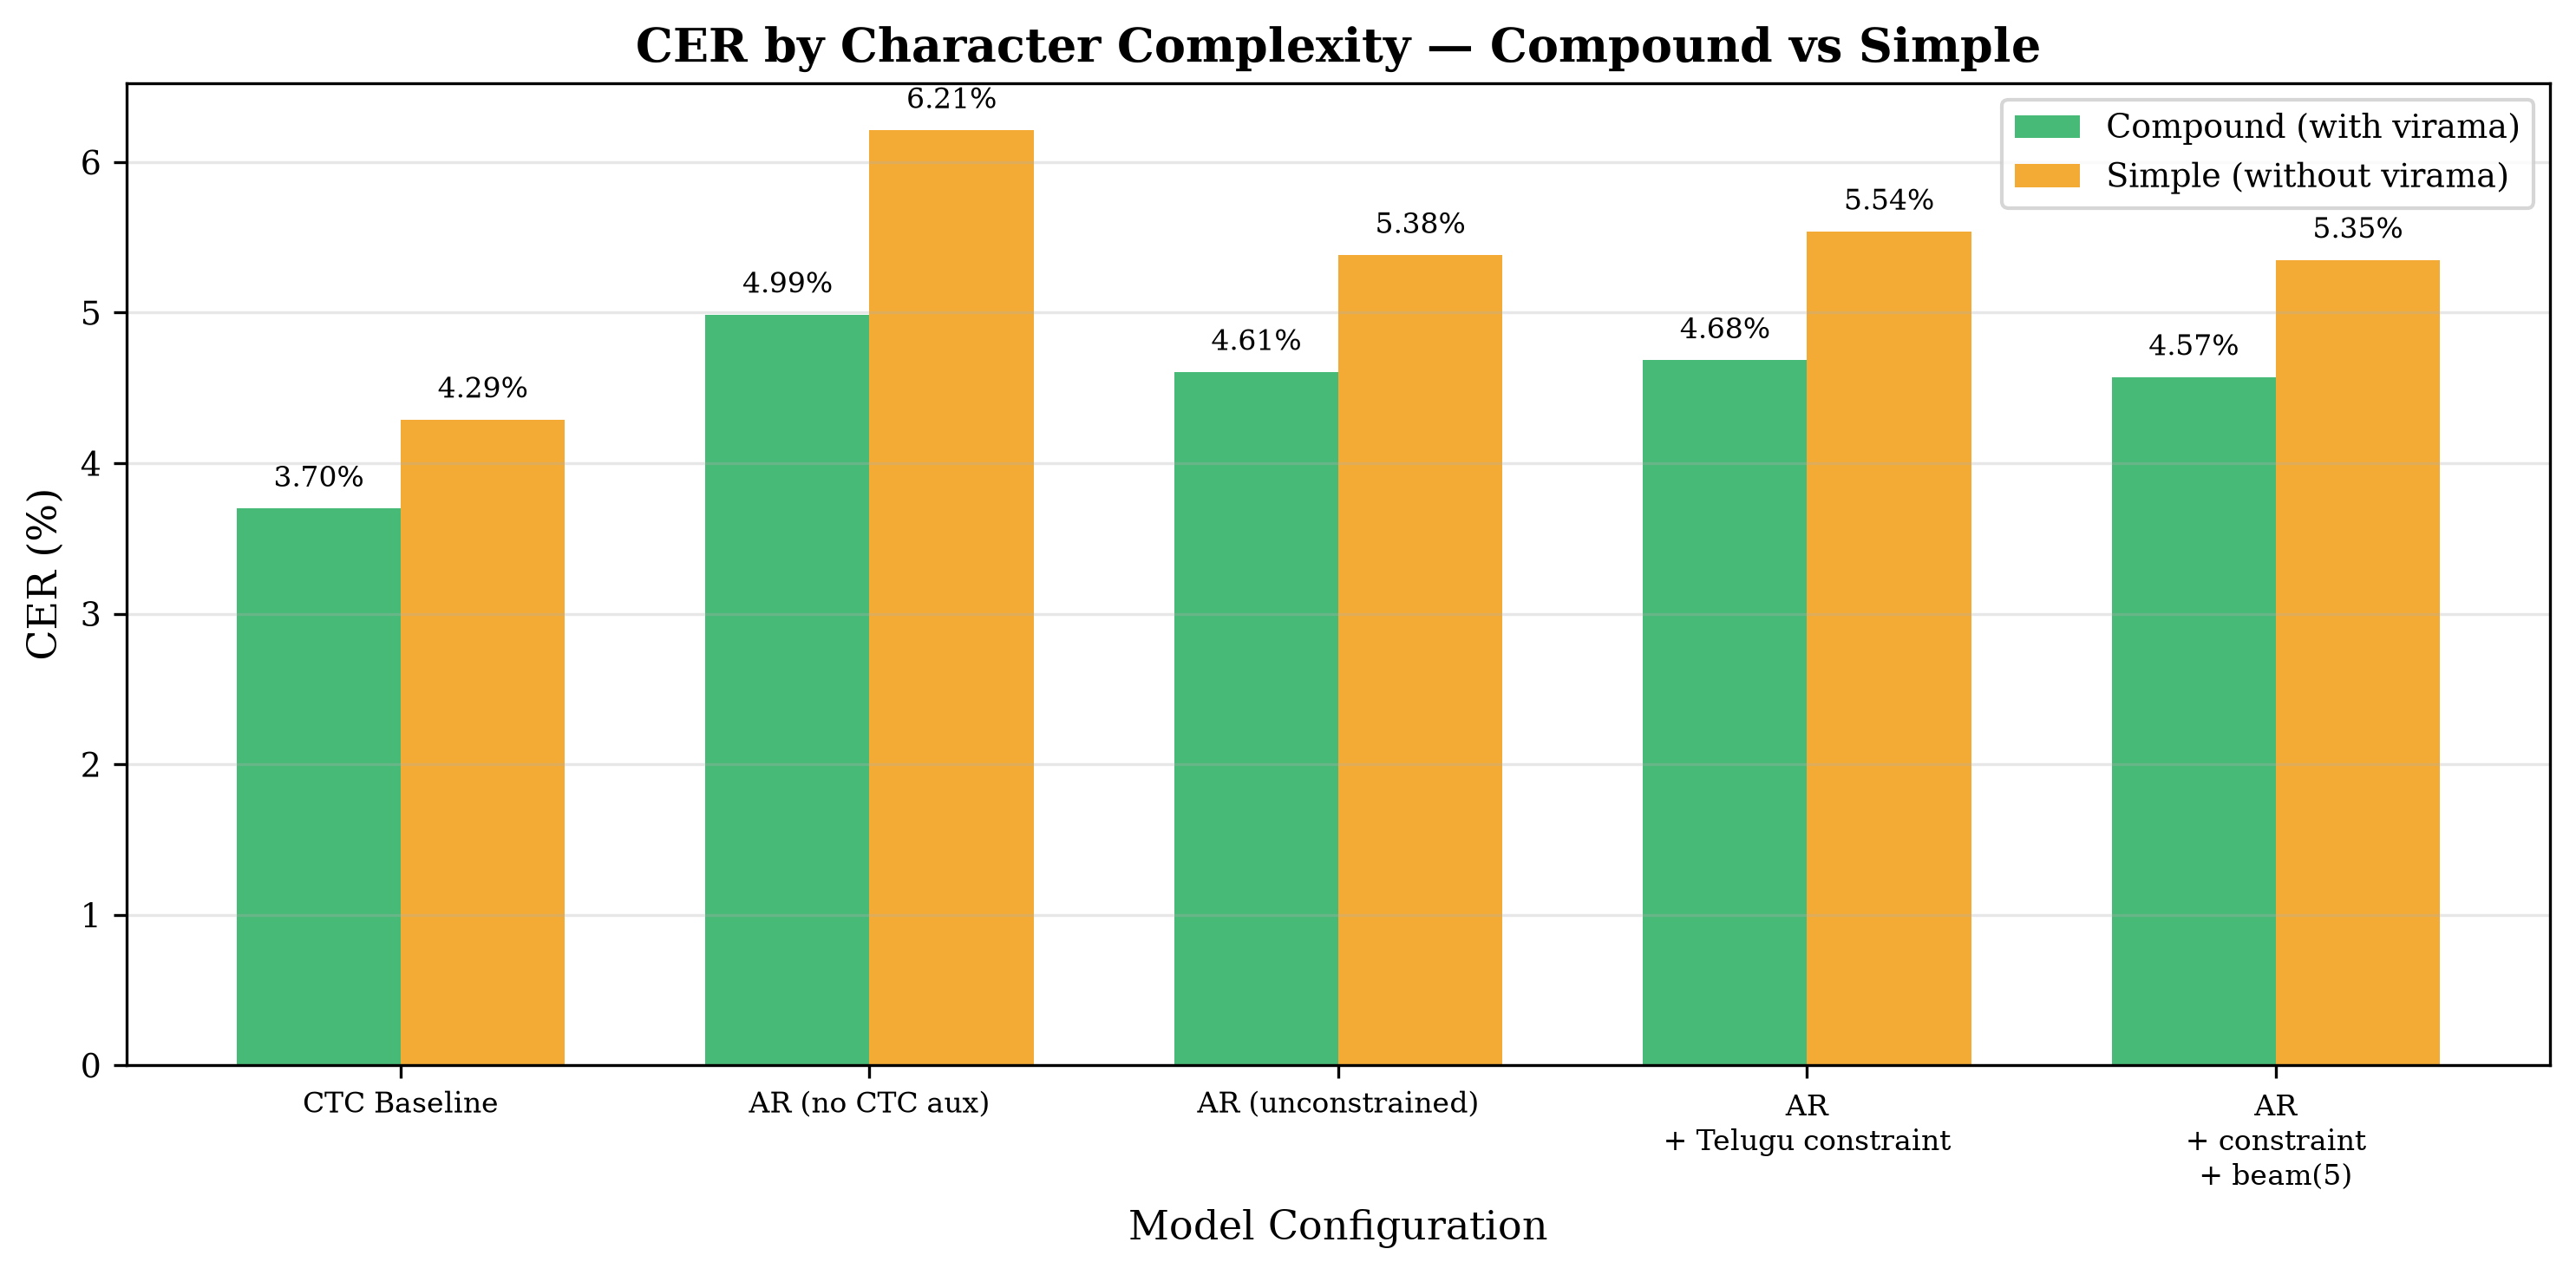
\includegraphics[width=\columnwidth]{figures/compound_vs_simple.png}
    \caption{CER comparison between compound characters (containing virama/conjuncts) and simple characters across all model variants. Compound characters are consistently recognized more accurately.}
    \label{fig:compound}
\end{figure}

We categorize test samples into \textit{compound} (containing at least one virama, $n = 10{,}129$) and \textit{simple} (no virama, $n = 7{,}781$) words. Fig.~\ref{fig:compound} presents the per-category CER.

Counter-intuitively, compound characters are recognized \textit{more} accurately (CER 3.70\%) than simple characters (CER 4.29\%) across all models. We hypothesize that compound forms create more visually distinctive glyph shapes, providing stronger discriminative features to the CNN encoder. Simple characters, particularly visually similar consonant-matra pairs, produce more ambiguous feature representations.

\subsection{Qualitative Error Analysis}

\begin{figure}[t]
    \centering
    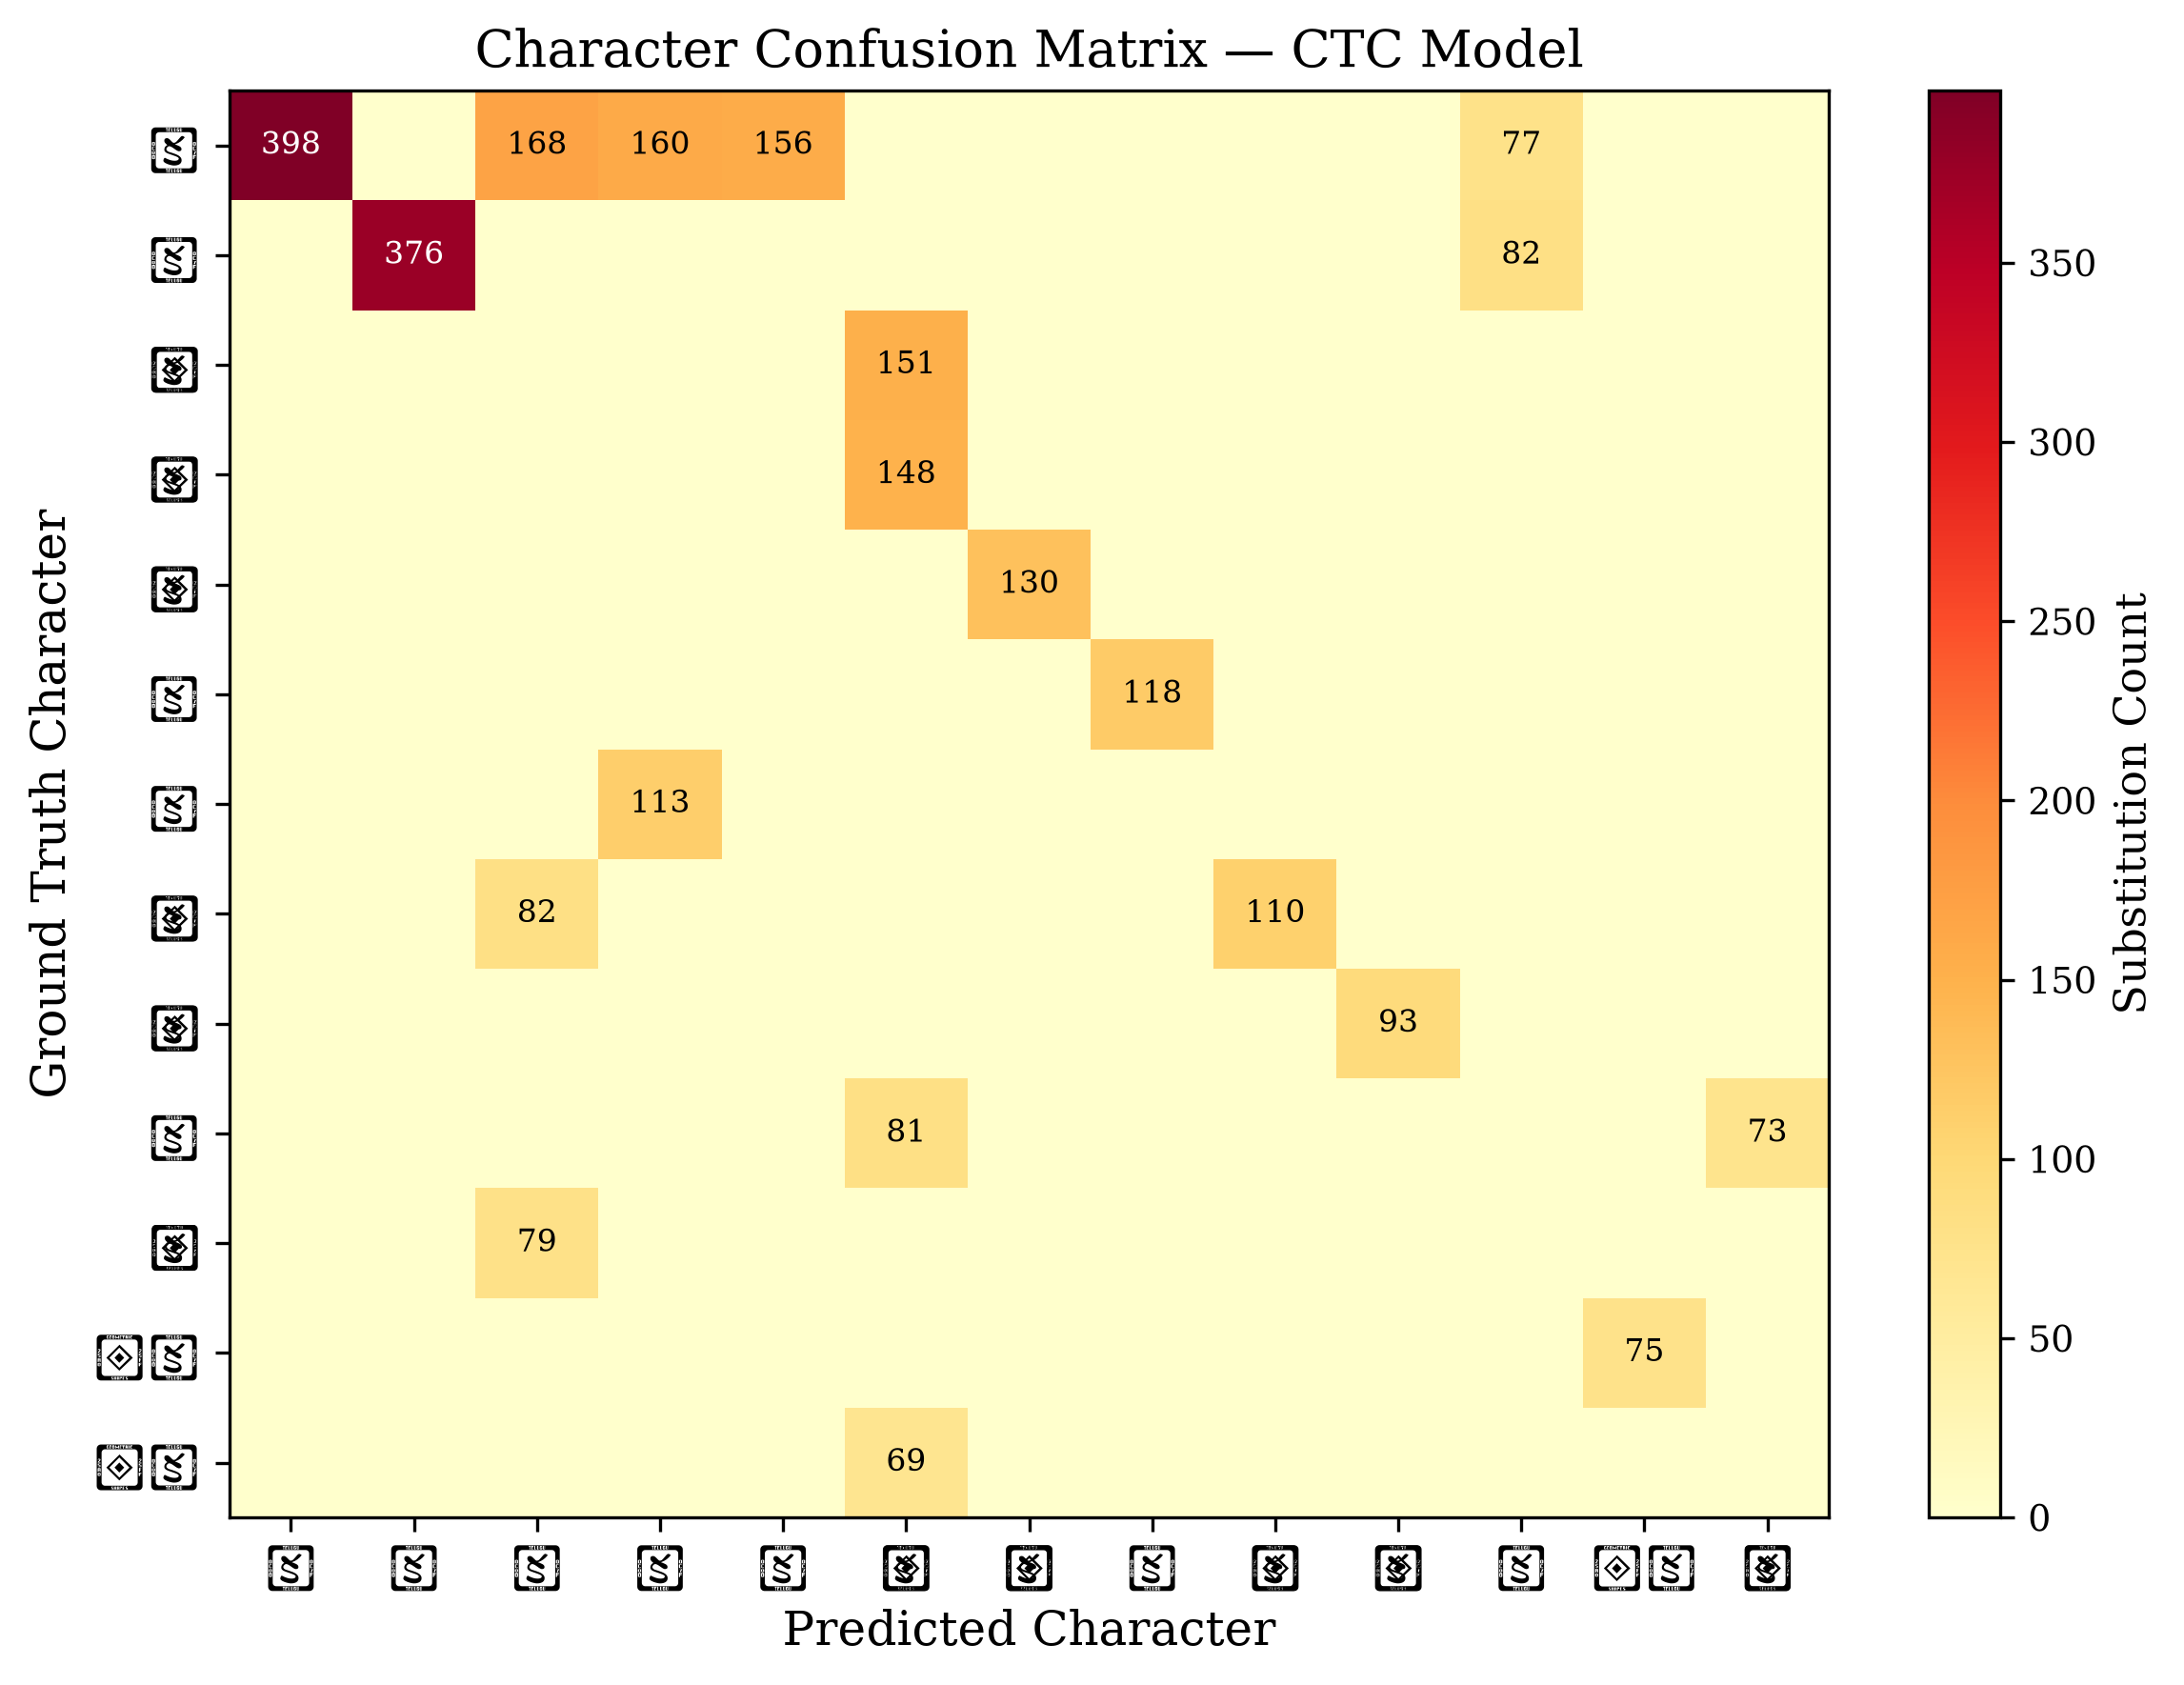
\includegraphics[width=\columnwidth]{figures/confusion_matrix_ctc.png}
    \caption{Character-level confusion matrix for the CTC baseline model, showing the top substitution errors. The most frequent confusions involve visually similar character pairs.}
    \label{fig:confusion}
\end{figure}

Fig.~\ref{fig:confusion} presents the character-level confusion matrix for the CTC baseline. The most frequent substitution errors involve:

\begin{itemize}
    \item \textbf{Vowel sign confusion:} Short and long matra pairs (e.g., \textit{i-matra} vs.\ \textit{ii-matra}) that differ by a small visual stroke.
    \item \textbf{Consonant similarity:} Characters with shared stroke patterns (e.g., \textit{ga} vs.\ \textit{da}) where the distinguishing feature is subtle.
    \item \textbf{Numeral confusion:} Telugu numerals (e.g., \textit{35}) being misrecognized as character sequences with similar stroke patterns.
\end{itemize}

These error patterns suggest that higher-resolution feature extraction or character-level attention mechanisms could yield further improvements.

\subsection{Statistical Significance}

Statistical significance is assessed via non-overlapping bootstrap 95\% CIs. The CTC baseline [3.79\%, 4.03\%] and best AR variant [4.72\%, 5.00\%] have non-overlapping intervals, confirming the CTC model's superiority is statistically significant ($p < 0.05$).

Conversely, AR greedy [4.75\%, 5.02\%] vs.\ AR beam search [4.72\%, 5.00\%] have fully overlapping intervals, indicating that beam search provides no statistically significant improvement despite a $192\times$ increase in inference latency (1.7~ms to 327.5~ms per sample).

% ═══════════════════════════════════════════════════════════════════
% VI. DISCUSSION
% ═══════════════════════════════════════════════════════════════════
\section{Discussion}

\subsection{Why CTC Outperforms the Transformer}

The superiority of the CTC baseline over Transformer-based decoders warrants analysis. We identify three factors:

\textbf{(1) Short sequence lengths.} The average word length in IIIT-HW-Telugu is 8.7 characters. Autoregressive decoders excel at modeling long-range dependencies in extended sequences (sentences, paragraphs), but for short words, the BiLSTM's bidirectional context provides sufficient modeling capacity.

\textbf{(2) Well-segmented inputs.} The test images are pre-segmented individual words. CTC's alignment-free nature is well-suited to this setting, whereas the Transformer decoder's cross-attention must learn word-level alignment from scratch---a task with limited benefit when spatial features are already well-ordered by the width-preserving encoder.

\textbf{(3) Training data scale.} Transformer architectures typically require larger datasets to realize their capacity advantages. With 80K training samples, the BiLSTM-CTC model may have a more favorable parameter-to-data ratio (13.1M vs.\ 17.3M parameters).

These findings suggest that for word-level Indic HTR with segmented inputs, CTC remains the recommended approach. Transformers may prove superior for line-level or page-level recognition where longer sequences and language modeling capabilities become critical.

\subsection{Linguistic Constraints: Marginal Impact}

The Telugu grammar mask provides only marginal and statistically insignificant improvements in accuracy. We attribute this to:

\begin{enumerate}
    \item The model already achieves low error rates ($<$5\% CER), leaving few errors for the constraint mask to correct.
    \item The data-driven bigram matrix may be overly permissive, allowing most transitions observed in training rather than encoding strict orthographic rules.
    \item The penalty-based approach ($\alpha = 10.0$) is a soft constraint that does not guarantee grammaticality, unlike hard masking.
\end{enumerate}

Future work could explore grammar masks derived from formal Telugu phonological rules, or integration with character-level language models for more effective linguistic reasoning.

\subsection{Threats to Validity}

\textbf{Internal validity.} The linguistic constraint matrix is constructed from training set bigram statistics rather than formal Telugu grammar rules. Rare but valid character sequences absent from the training data may be incorrectly penalized during constrained decoding.

\textbf{External validity.} The IIIT-HW-Telugu dataset contains segmented word images; results may not generalize to unconstrained page-level recognition where word segmentation errors compound. The dataset contains modern Telugu handwriting; performance on historical manuscripts or significantly degraded documents is untested. Cross-dataset evaluation on additional Telugu corpora (e.g., CHIPS) would further strengthen generalizability claims.

\textbf{Construct validity.} CER and WER are computed at the word level. For practical deployment, sentence-level or paragraph-level metrics with a language model would be more representative of real-world performance. Inference speed measurements include only GPU computation time and exclude I/O, preprocessing, and postprocessing overhead.

% ═══════════════════════════════════════════════════════════════════
% VII. CONCLUSION AND FUTURE WORK
% ═══════════════════════════════════════════════════════════════════
\section{Conclusion}

We presented a comprehensive study of CTC and Transformer-based architectures for Telugu handwritten text recognition on the IIIT-HW-Telugu benchmark. Our modified ResNet-18 encoder with width-preserving feature extraction, combined with a BiLSTM-CTC decoder, achieves 3.91\% CER---a new state-of-the-art for lexicon-free Telugu HTR, representing a 39\% relative improvement over prior work.

Our ablation study yields three key insights: (1)~auxiliary CTC loss is essential for training autoregressive Transformer decoders on Indic HTR tasks, providing a 10\% relative CER reduction; (2)~CTC baselines outperform Transformer decoders on well-segmented word-level recognition tasks with short sequences; and (3)~data-driven Telugu linguistic constraints provide minimal accuracy improvements at current error rates, suggesting that the model already captures most orthographic patterns implicitly.

\textbf{Future work} will explore: (a)~line-level and page-level recognition where Transformers' language modeling capabilities are expected to provide greater advantages; (b)~formal phonology-based grammar masks derived from Telugu linguistic rules; (c)~pre-training on synthetic Telugu text data generated from Unicode fonts; and (d)~cross-script transfer learning leveraging shared Brahmic script features across Telugu, Kannada, Tamil, and other Dravidian languages.

% ═══════════════════════════════════════════════════════════════════
% REPRODUCIBILITY
% ═══════════════════════════════════════════════════════════════════
\section*{Reproducibility}

All source code, configuration files, and training scripts are publicly available at \url{https://github.com/[your-username]/telugu-htr}. The software stack comprises Python~3.12.13, PyTorch~2.7.1 (CUDA~11.8, cuDNN~9.1.0) on Ubuntu~22.04. All experiments were conducted on a single NVIDIA RTX~3090~Ti (24~GB). Total training time: $\sim$9.5 hours. The IIIT-HW-Telugu dataset is available at \url{https://cvit.iiit.ac.in/research/projects/cvit-projects/indic-hw-data}.

% ═══════════════════════════════════════════════════════════════════
% REFERENCES
% ═══════════════════════════════════════════════════════════════════
\bibliographystyle{IEEEtran}

\begin{thebibliography}{20}

\bibitem{vaswani2017attention}
A.~Vaswani, N.~Shazeer, N.~Parmar, J.~Uszkoreit, L.~Jones, A.~N.~Gomez, {\L}.~Kaiser, and I.~Polosukhin, ``Attention is all you need,'' in \textit{Proc. Advances in Neural Information Processing Systems (NeurIPS)}, vol.~30, 2017, pp.~5998--6008.

\bibitem{graves2006ctc}
A.~Graves, S.~Fern{\'a}ndez, F.~Gomez, and J.~Schmidhuber, ``Connectionist temporal classification: Labelling unsegmented sequence data with recurrent neural networks,'' in \textit{Proc. Int. Conf. Machine Learning (ICML)}, 2006, pp.~369--376.

\bibitem{he2016resnet}
K.~He, X.~Zhang, S.~Ren, and J.~Sun, ``Deep residual learning for image recognition,'' in \textit{Proc. IEEE Conf. Computer Vision and Pattern Recognition (CVPR)}, 2016, pp.~770--778.

\bibitem{li2023trocr}
M.~Li, T.~Lv, J.~Chen, L.~Cui, Y.~Lu, D.~Florencio, C.~Zhang, Z.~Li, and F.~Wei, ``TrOCR: Transformer-based optical character recognition with pre-trained models,'' in \textit{Proc. AAAI Conf. Artificial Intelligence}, vol.~37, 2023, pp.~13094--13102.

\bibitem{bautista2022parseq}
D.~Bautista and R.~Atienza, ``Scene text recognition with permuted autoregressive sequence models,'' in \textit{Proc. European Conf. Computer Vision (ECCV)}, 2022, pp.~178--196.

\bibitem{shi2017crnn}
B.~Shi, X.~Bai, and C.~Yao, ``An end-to-end trainable neural network for image-based sequence recognition and its application to scene text recognition,'' \textit{IEEE Trans. Pattern Analysis and Machine Intelligence}, vol.~39, no.~11, pp.~2298--2304, 2017.

\bibitem{puigcerver2017}
J.~Puigcerver, ``Are multidimensional recurrent layers really necessary for handwritten text recognition?,'' in \textit{Proc. Int. Conf. Document Analysis and Recognition (ICDAR)}, 2017, pp.~67--72.

\bibitem{scheidl2018word}
H.~Scheidl, S.~Fiel, and R.~Sablatnig, ``Word beam search: A connectionist temporal classification decoding algorithm,'' in \textit{Proc. Int. Conf. Frontiers in Handwriting Recognition (ICFHR)}, 2018, pp.~253--258.

\bibitem{dutta2018}
K.~Dutta, P.~Krishnan, M.~Mathew, and C.~V.~Jawahar, ``Towards accurate handwritten word recognition for Hindi and Bangla,'' in \textit{Proc. Int. Conf. Computer Vision Theory and Applications (VISAPP)}, 2018, pp.~470--477.

\bibitem{gongidi2021iiit}
S.~Gongidi and C.~V.~Jawahar, ``IIIT-INDIC-HW-WORDS: A dataset for Indic handwritten text recognition,'' in \textit{Proc. Int. Conf. Document Analysis and Recognition (ICDAR)}, 2021, pp.~444--459.

\bibitem{deshpande2021}
A.~Deshpande, P.~Krishnan, and C.~V.~Jawahar, ``Attention-based approaches for handwritten text recognition in Indic scripts,'' in \textit{Proc. Int. Workshop on Document Analysis Systems}, 2021.

\bibitem{platter2025}
A.~Namboodiri and S.~K.~Ghosh, ``PLATTER: A page-level handwritten text recognition framework for Indic scripts,'' in \textit{Proc. Int. Conf. Document Analysis and Recognition (ICDAR)}, 2025.

\bibitem{ethnologue2024}
D.~M.~Eberhard, G.~F.~Simons, and C.~D.~Fennig, \textit{Ethnologue: Languages of the World}, 27th~ed. Dallas, TX: SIL International, 2024.

\bibitem{efron1993bootstrap}
B.~Efron and R.~J.~Tibshirani, \textit{An Introduction to the Bootstrap}. New York: Chapman \& Hall, 1993.

\bibitem{hwang2016character}
K.~Hwang and W.~Sung, ``Character-level language modeling with recurrent highway hypernetworks,'' in \textit{Proc. Advances in Neural Information Processing Systems (NeurIPS)}, 2016.

\bibitem{anderson2017guided}
P.~Anderson, B.~Fernando, M.~Johnson, and S.~Gould, ``Guided open vocabulary image captioning with constrained beam search,'' in \textit{Proc. Conf. Empirical Methods in Natural Language Processing (EMNLP)}, 2017, pp.~936--945.

\bibitem{shin2021grammar}
S.~Shin, S.~Kang, and S.~Lee, ``Grammar-based decoding for structured sequence labeling,'' in \textit{Proc. Annual Meeting of the Association for Computational Linguistics (ACL)}, 2021.

\bibitem{inc4_2024}
S.~Reddy and K.~Anand, ``Enhancing recognition of handwritten Telugu characters using deep learning,'' in \textit{Proc. IEEE Int. Conf. Contemporary Computing and Communications (InC4)}, 2024, pp.~1--6.

\end{thebibliography}

\end{document}
